\section{Evaluation}
\label{sec:eval}

The evaluation asks three questions. Does the loop make real progress on a target it has not seen?
Does the commit rule keep the lineage honest? And what does a turn cost? All numbers below come from
transcripts committed in the repository (\file{evidence/}) and from the design log
(\file{PLAN.md}).

\subsection{Benchmarks}
\label{sec:eval-bench}

The repository ships two targets in \file{bench/}, chosen to be unlike each other
(\cref{tab:bench}). \cmd{fuzzysearch} is a speed problem with a known answer, so it tests the
harness. \cmd{arcagi3} is an open capability problem, so it tests the loop. A script copies a target
into a fresh git repository and refuses any path inside the avocode checkout, because \avo{commit}
would otherwise write the loop's lineage into avocode's own history.

\begin{table}[t]
\centering\small
\caption{The two benchmark targets. Both use \cmd{reduce = "dominate"}.}
\label{tab:bench}
\begin{tabularx}{\linewidth}{@{}l X X c c c@{}}
\toprule
Target & Task & \cmd{primary} & Dir. & Configs & $\varphi$ \\
\midrule
\cmd{fuzzysearch} & all (query, word) pairs with Levenshtein distance $\leq k$ & mean of per-config median ms per search & $\downarrow$ & 2 & 0.03 \\
\cmd{arcagi3} & play ARC-AGI-3 games \citep{arcprize2026arcagi3} from $64{\times}64$ frames & mean fraction of levels completed & $\uparrow$ & 10 & 0.1 \\
\bottomrule
\end{tabularx}
\end{table}

\paragraph{\cmd{fuzzysearch}.} Two configs, \cmd{small} (2{,}500 words, 80 queries) and
\cmd{large} (5{,}000 words, 120 queries), both with $k = 2$, are built from a seeded pseudo-lexicon
so they are identical on every machine. The repetition count adapts to the candidate's speed. Spread
is measured as an interquartile range, because max-minus-min showed 51\% ``spread'' at the fast end
from one garbage-collection pause. The seed program is a full dynamic-programming matrix built from
nested arrays: correct and slow. The scorer's \cmd{correct} has three gates, in order:
\begin{enumerate}[leftmargin=*,itemsep=1pt]
  \item \textbf{Hash gate}: \cmd{sha256sum -c} over the protected files (the reference, corpus,
    runner, unit tests, the scorer and the protected list itself).
  \item \textbf{Unit suite}: empty inputs, $k=0$, exact distances, Unicode, duplicates.
  \item \textbf{Full-scale check}: compare the candidate with an independent reference on the
    exact input that is timed, and check that the candidate did not mutate its arguments.
\end{enumerate}
Gate~3 matters. The end-to-end suite ships a candidate that passes every unit test but returns
nothing for corpora over 1{,}000 words. Only gate~3 catches it (``306 pair(s) missing''). An agent
that edits both the scorer and the hash file can defeat the in-repo gate, so an external
\cmd{bench/init.sh --verify} audits the protected files from outside the target after each run.

Before any agent ran, six hand-written versions (the \emph{ladder}) were replayed through
\avo{score} and \avo{commit} to prove that the target has headroom: two-row DP, length prefilter,
prefix/suffix trim, an Ukkonen band, a length-bucketed index, and a letter-set bitmask. All six
committed, and the ladder went from \SI{1719}{ms} to \SI{0.931}{ms} ($1847\times$) in the committed
transcript. A first candidate target, matrix multiplication, was rejected at this stage: five
classical optimizations gave only $1.7\times$ in total, because the V8 JIT already does that work.

\paragraph{\cmd{arcagi3}.} A policy plays ten offline ARC-AGI-3 games with a budget of 250 actions
per episode and 24 seeded rollouts per game. Games were removed if their baseline was zero, if they
were not reproducible (a real-time game scored 0.483, 0.533 and 0.483 on identical code), or if they
were saturated. The scorer adds a sandbox through Python audit hooks that refuses network access and
reads of the game files while the policy acts. An earlier version raised a plain \cmd{Exception},
and ``a policy wrapping its body in \texttt{except Exception: pass} swallowed the violation and
scored a clean 0.26''. Eight held-out games and the official API are scored outside $\f$, because
memorization is the one thing $\f$ cannot catch. A scripted two-rung ladder moves the training score
from 0.277 to 0.320 and the holdout from 0.217 to 0.227; its second rung is refused because one game
drops by 100\%. \textbf{No agent run on \cmd{arcagi3} is recorded}, so we report it as a built and
gated target, not as a result.

\subsection{Setup of the agent runs}

Both runs used \avo{run --agent claude} with Claude Code's default model on one workstation. $\K$
was seeded with four notes written offline: Ukkonen's banded DP, Myers' bit-parallel algorithm,
BK-trees with Levenshtein automata, and V8 numeric-loop performance. The notes ``deliberately do not
contain the ladder''. qmd and web search were not available, so $\K$ used the local-scan fallback. A
watchdog created \file{.avo/STOP} after a fixed time (1{,}500\,s for run~1, 1{,}200\,s for run~2), so
\textbf{both runs stopped on the clock, not on convergence}. Run~2 resumed the lineage of run~1 with
the same prompt. Before it started, the operator removed run~1's refused candidate from the working
tree and saved it as evidence. \Cref{tab:runs} lists the settings.

\begin{table}[t]
\centering\small
\caption{Settings and outcomes of the two agent runs on \cmd{fuzzysearch}.}
\label{tab:runs}
\begin{tabular}{@{}lcc@{}}
\toprule
 & Run 1 & Run 2 (resumed) \\
\midrule
Turns (budget)            & 6 (12) & 3 (6) \\
Per-turn timeout          & 480\,s & 900\,s \\
Wall-clock                & 34\,min 43\,s & 30\,min 41\,s \\
Stopped by                & watchdog & watchdog \\
Versions committed        & 4 (v1--v4) & 3 (v5--v7) \\
Refusals                  & 1 & 0 \\
Supervisor interventions  & 0 & 0 \\
Cost                      & $\geq$ \$1.91 (2 of 6 turns recoverable) & \$8.19 (\$2.73/turn) \\
$\f$ intact (external audit) & pass & pass \\
\bottomrule
\end{tabular}
\end{table}

\subsection{Results}

\Cref{tab:lineage,fig:results} give the lineage. Seven versions took the median search time from
\SI{1810.37}{ms} to \SI{0.231}{ms}, a $7837\times$ speedup, in nine turns and about 65 minutes of
agent time. Run~1 alone reached $5255\times$ in four versions. Every version satisfied
\cref{def:commit} against its parent with $\varphi = 3\%$, so no regression beyond the floor
was committed on either config.

\begin{table}[t]
\centering\small
\caption{The agent lineage on \cmd{fuzzysearch}. Times are medians in ms at commit time. Speedups
for v5--v7 versus v0 are computed by hand from the recorded primaries; the run transcript's ``vs
v0'' column is wrong for run~2 (it uses the run's start as v0).}
\label{tab:lineage}
\begin{tabularx}{\linewidth}{@{}c c X r r r r r@{}}
\toprule
Ver. & Run & Technique (from the commit rationale) & \cmd{small} & \cmd{large} & \cmd{primary} & vs.\ prev & vs.\ v0 \\
\midrule
v0 & -- & full DP matrix, nested arrays (seed) & -- & -- & 1810.37 & -- & $1\times$ \\
v1 & 1 & rolling \cmd{Int32Array} Ukkonen band, length-bucketed corpus, flat code units & 3.447 & 10.261 & 6.854 & $264.1\times$ & $264\times$ \\
v2 & 1 & character-set bitmask prefilter before the banded DP & 0.435 & 0.849 & 0.642 & $10.7\times$ & $2820\times$ \\
v3 & 1 & \textbf{partition (pigeonhole) hash index} --- not in the ladder & 0.309 & 0.507 & 0.408 & $1.57\times$ & $4437\times$ \\
v4 & 1 & PassJoin position-aware probe window on that index & 0.253 & 0.436 & 0.345 & $1.18\times$ & $5255\times$ \\
v5 & 2 & one interleaved \cmd{Int32Array} for the index & 0.248 & 0.413 & 0.331 & $1.04\times$ & $5478\times$ \\
v6 & 2 & Myers bit-parallel for survivors; layout fused into index build & 0.173 & 0.368 & 0.270 & $1.22\times$ & $6693\times$ \\
v7 & 2 & no flat corpus buffer; branchless Myers with early exit & 0.158 & 0.304 & 0.231 & $1.17\times$ & $7837\times$ \\
\bottomrule
\end{tabularx}
\end{table}

\begin{figure}[t]
\centering
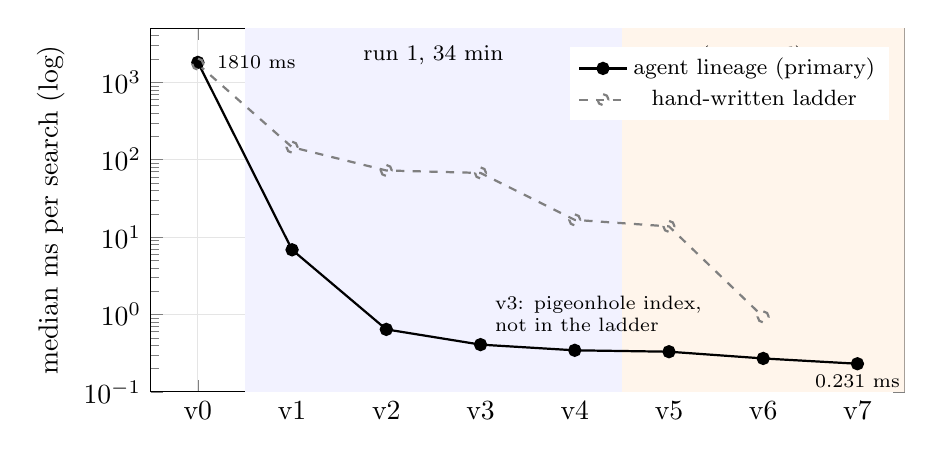
\begin{tikzpicture}
\begin{semilogyaxis}[
  width=0.92\linewidth, height=6.2cm,
  xmin=-0.5, xmax=7.5, ymin=0.1, ymax=5000,
  xtick={0,...,7}, xticklabels={v0,v1,v2,v3,v4,v5,v6,v7},
  ylabel={median ms per search (log)},
  grid=major, grid style={gray!20},
  legend style={at={(0.98,0.95)}, anchor=north east, font=\footnotesize, draw=none},
  every axis plot/.append style={thick},
]
  \fill[blue!5] (axis cs:0.5,0.1) rectangle (axis cs:4.5,5000);
  \fill[orange!8] (axis cs:4.5,0.1) rectangle (axis cs:7.5,5000);
  \node[font=\footnotesize, anchor=north] at (axis cs:2.5,4000) {run 1, 34 min};
  \node[font=\footnotesize, anchor=north] at (axis cs:6,4000) {run 2 (resumed), 31 min};
  \addplot[mark=*, black] coordinates
    {(0,1810.37) (1,6.854) (2,0.642) (3,0.408) (4,0.3445) (5,0.3305) (6,0.2705) (7,0.231)};
  \addlegendentry{agent lineage (\cmd{primary})}
  \addplot[mark=o, gray, dashed] coordinates
    {(0,1719.368) (1,145.093) (2,72.603) (3,67.434) (4,16.693) (5,13.7455) (6,0.931)};
  \addlegendentry{hand-written ladder}
  \node[font=\scriptsize, anchor=south west, align=left] at (axis cs:3.05,0.45)
    {v3: pigeonhole index,\\ not in the ladder};
  \node[font=\scriptsize, anchor=west] at (axis cs:0.1,1810) {1810 ms};
  \node[font=\scriptsize, anchor=north] at (axis cs:7,0.22) {0.231 ms};
\end{semilogyaxis}
\end{tikzpicture}
\caption{The \cmd{fuzzysearch} lineage on a log scale ($7837\times$, no committed regression). The
dashed line is the hand-written ladder from a separate transcript, shown for scale; its v0 is a
different measurement of the same seed. The ladder's last rung (\SI{0.931}{ms}) is slower than the
agent's v2.}
\label{fig:results}
\end{figure}

\paragraph{Reproduction.} An audit script re-measured every version from its own commit in a
detached worktree. All fresh measurements were slower than the recorded ones, by 0.9\% to 12.9\%,
all in one direction, because ``the box was busy''. The audit's pass band is 50\%, so all seven
versions passed. The audit also confirmed a monotone best and an intact $\f$.

\subsection{Case studies}

\paragraph{A step outside the ladder.} v1 fused five of the six ladder steps into one commit, and v2
matched the ladder's last step. v3 went further. The agent cut each corpus word into $k+1$ disjoint
segments and hashed them. By the pigeonhole principle, any match within $k$ edits keeps at least one
segment intact, so the scan becomes a few hash probes. A source comment records that this cut the
candidates from about 283k to about 23k on the scored workload. The commit rationale cites the
bucketing note in $\K$: ``the same idea applies to any filter whose key is discrete''. v4 (PassJoin
windows), v6 (Myers bit-parallel) and v7 also go beyond the ladder. The design log concludes that
``the ladder is a floor on this target, not a ceiling''. We note that the seeded notes named the
relevant algorithm families, so $\K$ shaped this result.

\paragraph{The one refusal.} In run~1, turn~6 (which hit the 480\,s timeout) left a candidate that
interleaved the index entries. It was slower than v4 on \cmd{small} by 4.74\%, outside the 3\%
floor, and the rule refused it: \emph{``\,`small' regressed (worst: small $-4.74\%$) (floor
$\pm3.00\%$)''}. In run~2, a fresh agent reached the same idea and made it win as v5: a tie on
\cmd{small} ($+2.0\%$, inside the floor) and a gain on \cmd{large} ($+5.3\%$). The dead-end record
did not block a better implementation of the same idea. It only blocked the version that
regressed.

\paragraph{A wrong note, corrected by measurement.} Each turn of run~2 started by measuring. The
turn that produced v6 timed each phase and found that the banded DP took 30--43\% of the call. Notes
from v4 and v5 had called it ``almost certainly too small to matter now''. The agent recorded that
the earlier note was wrong.

\paragraph{The rule shapes the step.} Two of the three turns in run~2 bundled changes on purpose. A
change worth $+2.66\%$ is inside the 3\% floor, so it cannot commit alone, and the agent shipped it
with a partner. The design log calls this ``the commit rule shaping the variation step''. It also
conflicts with the skill's ``one idea per candidate'' rule, which \cref{sec:discussion} discusses.

\paragraph{A dead end found twice.} The turns for v6 and v7 both tried to drop a counting sort and
both measured a regression. The second turn retried on purpose, reasoning that a later change should
have removed the first cause. It had not.

\subsection{Cost and tokens}
\label{sec:eval-cost}

Run~2 used 158 uncached input tokens, 119{,}912 output tokens, 5{,}555{,}257 cache-read tokens and
241{,}350 cache-write tokens, for \$8.19 or \$2.73 per turn. At that rate, the default budget of
12 turns costs about \$33, and \avo{run} has no cost cap. Run~1's cost is only a floor. Its
manifest recorded 44 of 985{,}039 input tokens (0.0045\%) because of two bugs: the parser read only
uncached input, and the output cap kept the head of the agent's stream while Claude Code writes usage
and cost in the last event. Four of six logs lost that event. Both bugs are fixed, and a replay tool
re-parses saved logs with the fixed parser. Bugs like this one, and an agent's own commits not being
credited to its turn, appeared only in real runs; stub agents in the test suite did not expose them.

\subsection{Engineering validation}

The repository has 441 unit tests (\cmd{node:test}, about 4.6\,s) and 14 end-to-end suites that run
the real \cmd{bin/avo} against temporary git repositories with a stub agent. Each suite writes a
transcript to \file{evidence/}; the current transcripts hold 496 passing checks. Continuous
integration runs lint, type checks, the unit tests and the end-to-end suites on every pull request,
with no agent installed on purpose. Examples of what the suites pin down: the stall fires at exactly
$N$ attempts and not before; a directive is appended to the turn prompt, not substituted; six
worsening scores in a pi session produce \emph{one} directive; a second \avo{install} produces no
diff; and a candidate that is fast but wrong at full scale fails $\f$.

The supervisor fired in these tests and \emph{never} in a real run. Across nine real turns,
attempts-since-best peaked at 2. ``A target with 5000x of headroom is improved faster than a stall
detector can notice one.''
